%% If you need to pass whatever options to xcolor
\PassOptionsToPackage{dvipsnames}{xcolor}

%% If you are using \orcid or academicons
%% icons, make sure you have the academicons 
%% option here, and compile with XeLaTeX
%% or LuaLaTeX.
% \documentclass[10pt,a4paper,academicons]{altacv}

%% Use the "normalphoto" option if you want a normal photo instead of cropped to a circle
% \documentclass[10pt,a4paper,normalphoto]{altacv}

\documentclass[10pt,a4paper]{altacv}

%% AltaCV uses the fontawesome and academicon fonts
%% and packages. 
%% See texdoc.net/pkg/fontawecome and http://texdoc.net/pkg/academicons for full list of symbols.
%% 
%% Compile with LuaLaTeX for best results. If you
%% want to use XeLaTeX, you may need to install
%% Academicons.ttf in your operating system's font 
%% folder.


% Change the page layout if you need to
\geometry{left=1cm,right=9cm,marginparwidth=6.8cm,marginparsep=1.2cm,top=1.25cm,bottom=1.25cm,footskip=2\baselineskip}

% Change the font if you want to.

% If using pdflatex:
\usepackage{hyperref}
\usepackage[utf8]{inputenc}
\usepackage[T1]{fontenc}
\usepackage{textcomp}
\usepackage[default]{lato}

\usepackage{skak}

% If using xelatex or lualatex:
% \setmainfont{Lato}

% Change the colours if you want to
\definecolor{Mulberry}{HTML}{72243D}
\definecolor{bahama blue}{HTML}{005B9A}
\definecolor{SlateGrey}{HTML}{2E2E2E}
\definecolor{LightGrey}{HTML}{666666}
\definecolor{Dark Slate Grey}{HTML}{2a4747}
\colorlet{heading}{Dark Slate Grey}
\colorlet{accent}{bahama blue}
\colorlet{emphasis}{SlateGrey}
\colorlet{body}{LightGrey}

% Change the bullets for itemize and rating marker
% for \cvskill if you want to
\renewcommand{\itemmarker}{{\small\textbullet}}
\renewcommand{\ratingmarker}{\faCircle}

%% sample.bib contains your publications
\addbibresource{sample.bib}
\title{Resume Fall 2019}
\begin{document}
\name{BRODY MCKEOWN}
\tagline{Electrical Engineering Co-op Student}
%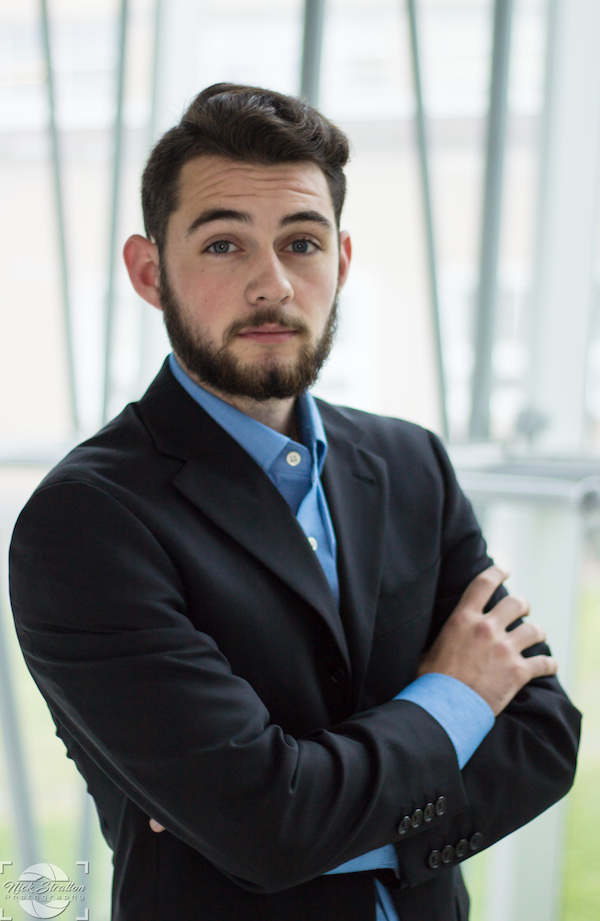
\includegraphics[width=\textwidth]{EngineeringHeadshot-2_copy.jpg}
%\photo{2.8cm}{Globe_High}
%\photo{3.5cm}{EngineeringHeadshot-2_copy.jpg}
\photo{3.5cm}{mysa.jpg}
%\photo{3.5cm}{test.jpg}
\personalinfo{%
  % Not all of these are required!
  % You can add your own with \printinfo{symbol}{detail}
  %\email{bmckeown@mun.ca}
   \email{\href{mailto:bmckeown@mun.ca}{bmckeown@mun.ca}}
  \phone{+1 (709) 690-4548}
  \location{St. John's, Newfoundland}
   \linkedin{\href{https://www.linkedin.com/in/brody-mckeown/}{brody-mckeown}}
  %% You MUST add the academicons option to \documentclass, then compile with LuaLaTeX or XeLaTeX, if you want to use \orcid or other academicons commands.
%   \orcid{orcid.org/0000-0000-0000-0000}
}

%% Make the header extend all the way to the right, if you want. 
\begin{fullwidth}
\makecvheader
\end{fullwidth}

%% Provide the file name containing the sidebar contents as an optional parameter to \cvsection.
%% You can always just use \marginpar{...} if you do
%% not need to align the top of the contents to any
%% \cvsection title in the "main" bar.

\cvsection[page1sidebar]{Experience}

\cvevent{Electrical Engineering Co-op Student}{Mysa Smart Thermostat}{April 2019 -- Aug 2019}{St.John's, Newfoundland}
\begin{itemize}
\item R\&D to bring new IoT product to market including market research, reverse engineering competitors' products and component testing
\item Made progress on and tested Embedded Systems in C
\item Developed temperature sensor test board in Altium
\end{itemize}

\divider

\cvevent{Hardware Design Engineering Co-op}{Curtiss-Wright Defense Solutions}{Sept 2018 -- Dec 2018}{Ottawa, Ontario}
\begin{itemize}
\item Executed Design Verification Testing on Single Board Computers using high speed oscilloscopes, phase noise analyzers and other laboratory equipment
\item Modified and repaired PCBs under a microscope
\item Performed circuit schematic and layout reviews  
\end{itemize}

\divider

\cvevent{Customer Applications Engineering Student}{Nokia}{Jan 2018 -- April 2018}{Ottawa, Ontario}
\begin{itemize}
\item Pro-actively troubleshooting problems in the proprietary network management software as well as customer networks and databases 
\item Worked with regional support teams, Research \& Development and product managers for technical support concerns
\item Developed Python scripts to aid in managing customers' network elements
\end{itemize}

\divider

\cvevent{Electrical Engineering Co-op Student}{Corner Brook Pulp \& Paper Mill}{May 2017 -- Sept 2017}{Corner Brook, Newfoundland}
\begin{itemize}
\item Updated and organized the motor management system and electrical equipment hierarchy utilizing JDEwards
\item Drafted mechanical parts and electrical drawings in AutoCAD
\item Developed work orders, budgets and procedures
\end{itemize}

\medskip

\cvsection{Education}
\cvevent{Bachelor of Electrical Engineering Co-op Program}{\faUniversity Memorial University of Newfoundland}{Sept 2016 -- Ongoing} {St.John's, Newfoundland}
Dean’s List 2016-2017 \hspace{0.125cm}%| \hspace{0.125cm}Academic Average 81\%
\linebreak Alfred and Annie Chan Electrical Engineering Scholarship 2017
\linebreak The PEGNL Engineering Scholarship 2017
\linebreak Expected Graduation: April 2021

\begin{comment}
\cvsection{Achievements}

\cvachievement{\hspace{0.125cm}\faBookmarkO}{Alfred and Annie Chan Electrical Engineering Scholarship}{2017}

%\cvachievement{\hspace{0.125cm}\faBookmarkO}{The Professional Engineers and Geoscientists of Newfoundland and Labrador Engineering Scholarship
%}{2017}


%\cvachievement{\hspace{0.125cm}\faBookmarkO}{Memorial University of Newfoundland Endowment Fund
%}{2017}

%\smallskip\divider\smallskip

%\cvachievement{\faTrophy}{Duke of Edinburgh’s Award Bronze \& Silver Standard}{2013, 2016}

\divider
\cvachievement{\faTrophy}{Provincial Chess Champion; Competitor at Canadian Chess Challenge}{2012-2015}
\smallskip
%\cvachievement{\faTrophy}{Canadian Chemistry Competition; First Place in Newfoundland}{2015}
\end{comment}
\clearpage

%% If the NEXT page doesn't start with a \cvsection but you'd
%% still like to add a sidebar, then use this command on THIS
%% page to add it. The optional argument lets you pull up the 
%% sidebar a bit so that it looks aligned with the top of the
%% main column.
% \addnextpagesidebar[-1ex]{page3sidebar}

\end{document}
